\section*{RESULTADOS}\label{sec:resultados}
\addcontentsline{toc}{section}{RESULTADOS}

Como se aprecia en el Cuadro \ref{tab:estrellas2} las imágenes IGRFJ17451 y MAXIJ1543 se obtuvieron de \cite{lopez2019quiescent} y luego de su respectivo análisis se obtuvo el Cuadro \ref{tab:estrellas}. \\

Para la primera estrella encontrada en IFRFJI17451 (véase Figura \ref{fig:estrella-rudik}) se determinó, por la suposición que se hizo, que la estrella tiene 0.99 $R_{\odot}$ y una luminosidad de 0.994 $L_{\odot}$ lo que la hace una estrella prácticamente igual al sol. Su tipo espectral es G2 y su clase de luminosidad es V. Su posición en el diagrama HR está en la secuencia principal. Es decir, una enana amarilla. \\

La zona habitable de está estrella, según \cite{lissauer_2020}, estaría entre 0.9 UA a 1.5 UA (al ser prácticamente igual al Sol). Lo que haría a la estrella potencialmente propensa a albergar vida, con las condiciones correctas de sus planetas que la orbitan. Por otro lado, los planetas que podría albergar esta estrella (basado las características del sol) serían gigantes gaseosos; los cuales podrían ser detectados por el método de imagen directa, tal y como se explica en \cite{bohn2020two}, en donde estudiaron un planeta similar al sol en el cual orbitan dos gigantes gaseosos.  \\

De la misma forma, para la estrella estudiada en MAXIJ1543, mostrada en la figura \ref{fig:estrella-bapt}, se estimó un radio de $0.8385 R_\odot$ y una luminosidad de $2.60 L_\odot$. La clasificación correspondiente sería K II. Como lo hemos supuesto, esta estrella pertenece a la secuencia principal. \\

Ya que esta estrella es más brillante y más caliente que el Sol, la zona habitable será un poco más lejos que la que existe alrededor de nuestra estrella. En unidades astronómicas (AU), se estima que iría de 0.95 AU hasta 1.676 AU. 
Ya que R=$0.8385 R_\odot$, se realizó una gráfica comparando los radios de las estrellas vs las masas de los planetas que los orbita.
\begin{figure}[ht]
    \centering
    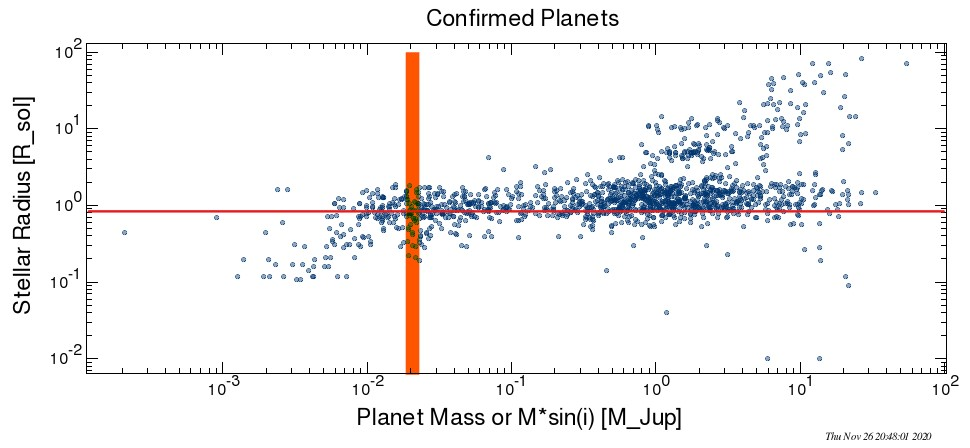
\includegraphics[scale=0.35]{Secciones/Radios.jpg}
    \caption{Radios estelares vs Masas de los planetas orbitando. }
    \label{fig:radios}
\end{figure}
En la Figura \ref{fig:radios}, obtenida de \cite{iceplotter_2020}, existen dos líneas: la horizontal indica la masa estimada de la estrella \ref{fig:estrella-bapt}. La línea vertical separa arbitrariamente los planetas con masas comparable a la de la Tierra (a la izquierda) y los planetas con masas comparables a la de Júpiter (a la derecha). Notamos que existen planetas comparables tanto a la Tierra como a Júpiter en la línea horizontal. A pesar de existir más planetas del tipo de Júpiter en la gráfica, podría ser un sesgo del sobreviviente: al graficar únicamente los planetas confirmados, y sabiendo de que es más fácil confirmar la existencia de planetas comparables a Júpiter, no podemos concluir nada más que puede existir cualquier clase de planeta orbitando a la segunda estrella.




